\section{Approach}
\label{sec:approach}

In this section, we present our agentic solution for the Text-to-Cypher task. We first describe the overall system architecture, highlighting the core components and their interactions. Then, we detail the design and implementation of the specific tools that enable our agent to effectively perform all the sub-tasks defined in Section \ref{sec:introduction}.

\subsection{System Architecture}

% include a figure of the architecture
\begin{figure}[h]
  \centering
  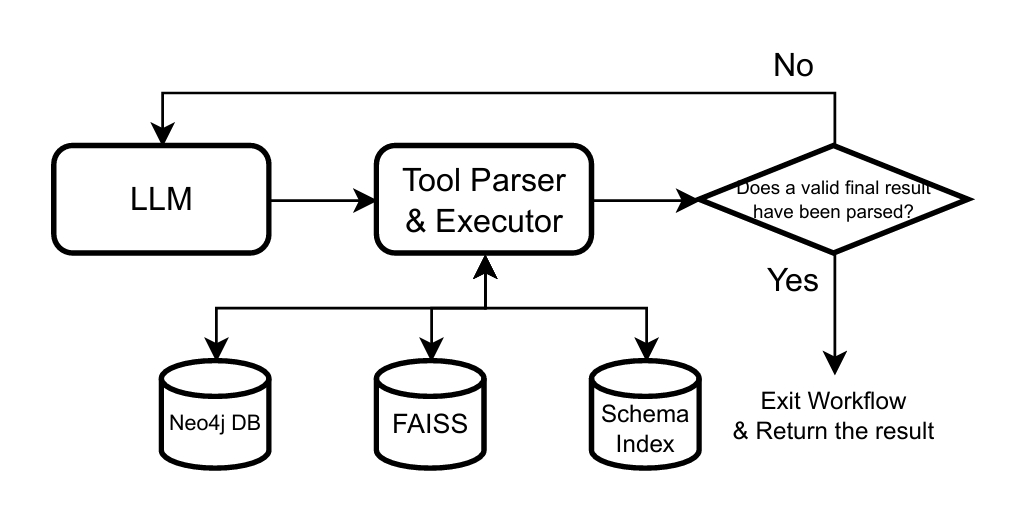
\includegraphics[width=0.8\linewidth]{./rsc/architecture.png}
  \caption{System Architecture}
  \label{fig:architecture}
\end{figure}


Our system is built upon the LangChain\footnote{\url{https://www.langchain.com/}} and LangGraph\footnote{\url{https://www.langchain.com/langgraph}} frameworks, which provide robust infrastructure for implementing stateful, multi-agent workflows. The architecture employs OpenAI's GPT-4.1 as the central reasoning engine, responsible for interpreting user queries and orchestrating the execution of sub-tasks necessary to generate the final Cypher query.

To enable \textbf{Relevant Formalisms Discovery}, the system incorporates a \textbf{FAISS Vector Store} \cite{faiss-douze-etal-2025} for semantic retrieval of schema components. This vector store indexes node labels, relationship types, and property keys from the target knowledge graph using the \href{https://huggingface.co/minishlab/potion-retrieval-32M}{minishlab/potion-retrieval-32M} Model2Vec embedding model, which is a finetuned version of the \href{https://huggingface.co/minishlab/potion-base-32M}{minishlab/potion-base-32M}\footnote{Which in turn it is a Model2Vec model distilled from the \href{https://huggingface.co/BAAI/bge-base-en-v1.5}{baai/bge-base-en-v1.5} Sentence Transformer \cite{xiao-etal-2023-cpack}} model

To capture the structural relationships between schema components, we designed a complementary \textbf{Schema Index}—an inverted index data structure that maintains bidirectional mappings between: (i) node labels and their properties, (ii) relationship types and their properties, (iii) relationship types and their valid domain-range node label pairs, (iv) property keys and their associated node labels, and (v) property keys and their associated relationship types. This index enables efficient reverse lookups and schema traversal queries.

The system operates through a ReAct-style agentic loop \cite{yao-etal-2023-react}, iteratively invoking tools and reasoning over observations until the agent either accumulates sufficient information to construct a valid Cypher query or determines that the user's question cannot be answered given the available knowledge graph.

\subsection{Tool Design and Implementation}

To enable the LLM agent to systematically perform the sub-tasks \ref{itm:discovery} and \ref{itm:linking} outlined in Section \ref{sec:introduction}, we designed a suite of specialized tools that facilitate efficient and effective schema exploration and information retrieval.%
%
\begin{minted}{python}
def search_for(
    components: List[Literal["nodes", "relationships", "properties"]],
    similar_to: str,
    top_k: int = 10
) -> str:
\end{minted}
%
The \verb|search_for| tool performs semantic search over the specified vector-indexed schema components (node labels, relationship types, and property keys) to identify all plausible candidate formalisms that could represent a given concept. The tool accepts three parameters: \verb|components| (specifying which schema component types are included in the search space), \verb|similar_to| (a natural language description of the concept), and \verb|top_k| (the number of results to return). This design explicitly prioritizes \textit{recall over precision}: the tool is intended to cast a wide net and retrieve all potentially relevant schema components, even at the cost of including some false positives. This design choice is crucial because missing a relevant schema component early in the retrieval process would be more costly to recover in subsequent steps, whereas false positives can be filtered out through later precision refinement, delegating it to subsequent tools. To maximize efficiency and minimizing latency, the tool is designed to be invoked in parallel for each independent concept within a complex query. Lastly, both here and in the subsequent tools, \verb|similar_to| and \verb|top_k| parameters are used to limit results only to the most relevant one avoiding polluting and consuming the LLM token context window with useless information.%
%
% \paragraph{Usage Pattern.}  For instance, consider the query: \textit{``Find all movies directed by someone who also acted in them, showing the budget and box office revenue''}. The agent decomposes this into four information needs: (i) movie entities, (ii) directors and their relationships, (iii) actors and their relationships, and (iv) financial data. Rather than sequential exploration, the agent issues four parallel \verb|search_for| calls with targeted similarity queries like \textit{``movie film production media''}, \textit{``director person directed manages leads''}, \textit{``actor person acted\_in performed starred cast''}, and \textit{``budget revenue earned cost''}.
%
\begin{minted}{Python}
def get_properties_from(
    components: List[Literal["nodes", "relationships"]],
    of_types: List[str],
    similar_to: Optional[List[str]] = None,
    top_k: Union[int, List[int]] = 10
) -> str:
\end{minted}
%
Once relevant node labels or relationship types have been identified, for each \textit{i-th} element in the batch, the \verb|get_properties_from| tool retrieves the associated properties of the schema component \verb|components[i]| of type \verb|of_types[i]| optionally ranked by similarity to \verb|similar_to[i]|. This \textit{batching-first} design philosophy is critical for two reasons: (i) it reduces the number of LLM tool calls, thereby decreasing latency and token consumption, and (ii) it encourages the agent to think holistically about multiple schema components simultaneously rather than myopically focusing on one at a time. %
%
% \paragraph{Usage Pattern.} Consider a query requiring employee information with their skills and company details. After identifying \verb|Person|, \verb|Company|, and \verb|Skill| nodes, rather than three separate calls, the agent batches them:
% \begin{minted}{python}
% get_properties_from(
%     components=["nodes", "nodes", "nodes"],
%     of_types=["Person", "Company", "Skill"],
%     similar_to=[
%         "employee name position salary",
%         "company industry sector revenue",
%         "skill expertise level"
%     ],
%     top_k=[10, 10, 8]
% )
% \end{minted}
%
\begin{minted}{Python}
def get_domains_ranges_of(
    relationships: List[str],
    similar_to: Optional[List[str]] = None,
    order_by: List[Literal["domains", "ranges"]] = None,
    top_k: Union[int, List[int]] = 10
) -> str:
\end{minted}
%
The \verb|get_domains_ranges_of| tool for each relationship type \verb|relationships[i]| retrieves valid pairs of domain (source) and range (target) node labels most similar to the \verb|similar_to[i]| query. The \verb|order_by[i]| parameter allows the agent to specify whether the ranking should be applied on domains or ranges. This tool is essential for understanding how different entities are interconnected within the graph, enabling the agent to reason about potential traversal paths and relationship chains necessary for constructing complex Cypher queries.%
%
% For example, in the query \textit{``Find people who invested in companies that were later acquired''}, the agent needs to understand the connection pattern: \verb|Person| → \verb|INVESTED_IN| → \verb|Company| → \verb|ACQUIRED| → \verb|Company|. By batching the exploration of \verb|INVESTED_IN| and \verb|ACQUIRED| relationships with appropriate \verb|similar_to| queries (\textit{``person investor individual''} for \verb|INVESTED_IN| domains and \textit{``company target acquired''} for \verb|ACQUIRED| ranges), the agent can efficiently validate the feasibility of the query path.
% \paragraph{Usage Pattern.} The batching paradigm applies here as well:
% \begin{verbatim}
% get_domains_ranges_of(
%     relationships=["INVESTED_IN", "ACQUIRED"],
%     similar_to=["person investor", 
%                 "company acquired target"],
%     order_by=["domains", "ranges"],
%     top_k=[5, 3]
% )
% \end{verbatim}
%
\begin{minted}{Python}
def get_components_with_property(
    keys: List[str],
    components: List[Literal["nodes", "relationships", "both"]],
    similar_to: Optional[List[str]] = None,
    top_k: Union[int, List[int]] = 10
) -> str:
\end{minted}
%
While most tools follow a forward lookup pattern (from schema components to properties), \verb|get_components_with_property| performs reverse lookup finding, for each property key \verb|keys[i]|, which schema components \verb|components[i]| most similar to the query \verb|similar_to[i]| possess it. This tool is particularly valuable for disambiguating queries where discriminative properties serve as strong signals for \textbf{Relevant Formalisms Discovery} (Sub-task \ref{itm:discovery}). %
%
% For example, in a query about \textit{``entities with creation timestamps''}, the property key \verb|created_at| is highly discriminative and can efficiently narrow down candidate node labels and relationship types.
% \paragraph{Usage Pattern.} Consider a temporal analysis query requiring entities with temporal information. Rather than guessing which entities might have timestamps, the agent can batch-query multiple temporal property keys:
% \begin{verbatim}
% get_components_with_property(
%     keys=["created_at", "timestamp", "since", "year"],
%     components=["both", "both", "relationships", "both"],
%     similar_to=["recent new", "event time",
%                 "employment duration", "temporal period"],
%     top_k=5
% )
% \end{verbatim}
% This reveals all schema components (nodes and relationships) that contain temporal properties, ranked by relevance to different temporal concepts.
%
\begin{minted}{Python}
def execute_cypher_query(cypher: str) -> List[dict]:
\end{minted}
%
The \verb|execute_cypher_query| tool provides a flexible mechanism for the agent to validate assumptions, explore data instances, and verify the existence of specific patterns through the execution of arbitrary Cypher queries. Unlike the schema-focused tools, this tool operates at the data instance level and, therefore, it is crucial for grounding the agent's schema-level reasoning in actual data instances, enabling it to confirm hypotheses that inform the final query construction. %
%
% \paragraph{Usage Pattern.} For instance, after identifying \verb|Person| nodes and \verb|WORKS_AT| relationships, the agent might execute:
% \begin{verbatim}
% execute_cypher_query(
%     "MATCH (p:Person)-[r:WORKS_AT]->(c:Company) 
%      RETURN p.name, r.since, c.name LIMIT 5"
% )
% \end{verbatim}
% This provides concrete examples of how these components are used in the actual graph, offering valuable context for query construction. The tool incorporates token-based truncation (default 4000 tokens) to prevent excessively large result sets from overwhelming the LLM's context window.
%
\begin{minted}{Python}
def register_retrieval_result(
    motivation: str,
    cypher_query: Optional[str] = None,
    kg_schema: Optional[KGSchema] = None
) -> RetrievalAgent.Result:
\end{minted}
%
The \verb|register_retrieval_result| tool allow the LLM to end the ReAct loop by summarizing the findings with a structured output containing: (i) the \verb|motivation| explaining why the user's query can or cannot be answered with a cypher query given the discovered schema components in the provided knowledge graph, (ii) optionally the constructed \verb|cypher_query|, and (iii) an optional \verb|kg_schema| object that encapsulates the discovered sub-schema relevant to the user's query. This structured output is essential for downstream components that may need to further process or execute the generated Cypher query.

This carefully orchestrated tool ecosystem enables the LLM agent to systematically navigate the complex space of schema exploration, moving from broad conceptual understanding to precise formal query construction while maintaining both comprehensiveness and efficiency.

